\documentclass[a4paper,12pt]{book}

%Pacchetti utili
%************
%* packages *
%************

%Codifica
\usepackage[utf8]{inputenc}

%Lingua, sostituire italian con english nel caso in cui la tesi sia scritta in inglese
\usepackage[italian]{babel}

%Titoli
\usepackage{titlesec}

%Pacchetto per definire layout di pagina
\usepackage{fancyhdr}
\usepackage{sectsty}
\usepackage[left=3cm, right=3cm, bottom=3cm]{geometry}

%Spazia linee all'interno del documento
\usepackage{setspace}

%Listati di codice
\usepackage{verbatim}
\usepackage{listings}

%Didascalie immagini
\usepackage[hang,small,sf,font=small, labelfont=bf]{caption}
\usepackage{subcaption}

%Inclusione immagini
\usepackage{graphicx}

%Impostazioni note a piè pagina
\usepackage[stable]{footmisc}

%Citazioni e riferimenti a label
\usepackage[english]{varioref}

%Colori
\usepackage[usenames]{color}
\usepackage{xcolor}
\usepackage{colortbl}

%Crea link ipertestuali
\usepackage[hidelinks]{hyperref}

\hypersetup{
            pdfauthor={Alberto Molon},
            pdftitle={Modelli di Code per la Descrizione del Processo di Mining di una Criptovaluta},
            pdfsubject={Information Security},
            pdfkeywords={Information Security, Teoria delle Code},
            pdfproducer={LaTex}
}

%Formattazione url
\usepackage{url}

%Inserimento formule
\usepackage{amsmath}
\usepackage{mathrsfs}
\usepackage{amssymb,amsthm}    % matematica
\theoremstyle{plain}
\newtheorem{teorema}{Teorema}

%Usato per diminuire spazio tra la parte superiore della pagina e l'indice
\usepackage{tocloft}

%Per avere tabelle più verso sx (soprattutto per quelle larghe)
\usepackage{changepage}

\usepackage{tabularx}

\usepackage[backend=biber,style=numeric,hyperref,backref]{biblatex}
                                        % eccellente pacchetto per la bibliografia; 
                                        % produce uno stile di citazione autore-anno; 
                                        % lo stile "numeric-comp" produce riferimenti numerici
                                        % per includerlo nel documento bisogna:
                                        % 1. compilare una prima volta Tesi.tex;
                                        % 2. eseguire da terminale: biber Tesi
                                        % 3. compilare ancora Tesi.tex.
\bibliography{bibliografia}

                                        
                                        



%Nuovi comandi
%*****************
%* nuovi comandi *
%*****************
\renewcommand{\&}{\textup{\symbol{`\&}}}
\newcommand{\abs}[1]{\left|#1\right|}                               % modulo
\newcommand{\dato}{\left|\right.}                                   % probabilit\`{a} condizionata
\newcommand{\fun}[1]{\mathrm{#1}}                                   % stile funzione
\newcommand{\imp}{\;\;\Longrightarrow\;\;}                          % implicazione
\newcommand{\norma}[1]{\left\| #1 \right\|}                         % norma
\newcommand{\prob}[1]{\mathrm{P}\!\left[#1\right]}                  % probabilit\`{a}
\newcommand{\expect}[1]{\mathrm{E}\!\left[#1\right]}                % aspettazione
\newcommand{\sse}{\;\;\Longleftrightarrow\;\;}                      % se e solo se
\newcommand{\vect}[1]{{\boldsymbol{\mathrm{#1}}}}                   % stile vettore
\newcommand{\real}[1]{\fun{Re}\left[#1\right]}                      % parte reale
\newcommand{\imag}[1]{\fun{Im}\left[#1\right]}                      % parte immaginaria
\newcommand{\Dim}[1]{\fun{dim}\left[#1\right]}                      % dimensione di una matrice
\newcommand{\Det}[1]{\fun{det}\left[#1\right]}                      % determinante di una matrice
\newcommand{\Ker}[1]{\fun{ker}\left[#1\right]}                      % ker di una matrice
\newcommand{\rango}[1]{\fun{rango}\left[#1\right]}                  % rango di una matrice
\newcommand{\scalare}[2]{\left\langle #1, #2 \right\rangle}         % prodotto scalare
\newcommand{\blbrace}{\left  \lbrace}                               % parentesi graffa sinistra grande
\newcommand{\brbrace}{\right \rbrace}                               % parentesi graffa destra grande
\newcommand{\sinc}{\fun{sinc}}                                      % sinc
\newcommand{\rect}{\fun{rect}}                                      % rect
\newcommand{\rcos}{\fun{rcos}}                                      % rcos
\newcommand{\sgn}{\fun{sgn}}                                        % sgn
\newcommand{\N}{\mathbb{N}}                                         % insieme dei numeri naturali
\newcommand{\Z}{\mathbb{Z}}                                         % insieme dei numeri interi
\newcommand{\Q}{\mathbb{Q}}                                         % insieme dei numeri razionali
\newcommand{\R}{\mathbb{R}}                                         % insieme dei numeri reali
%\newcommand{\C}{\mathbb{C}}                                         % insieme dei numeri complessi
\newcommand{\seq}[2][n]{#2_{0}, #2_{1}, \ldots, \, #2_{#1}}         % sequenza
\newcommand{\Span}[2][n]
{\fun{span} \blbrace #2_{1}, #2_{2}, \ldots, \, #2_{#1} \brbrace}   % spazio generato
\newcommand{\ddt}{\frac{\fun{d}}{\fun{dt}}}                         % derivata
\newcommand{\Div}[2]{#1 \; \mid \; #2}                              % divide
\newcommand{\MCD}[2]{\fun{MCD}\(#1, #2\)}                           % massimo comun divisore
\newcommand{\mcm}[2]{\fun{mcm}\(#1, #2\)}                           % minimo comune multiplo
\newcommand{\goodgap}{
                      \hspace{\subfigtopskip}
                      \hspace{\subfigbottomskip}
                     }                                              % interlinea opportuna per le sottofigure
\newcommand{\eng}[1]{\emph{#1}}                                   % inglese
\newcommand{\virg}[1]{``#1"}                                        % fa una citazione tra virgolette
%\newcommand{\unit}[2]($\frac{\text{#1}}{\text{#2}}$)                % unit\`{a} di misura
\newcommand{\textttvar}[1]{{\ttvar #1}}

\definecolor{gray}{gray}{0.9}
\newcommand{\listato}[1]{\lstset{language=#1, numbers=left, numberstyle=\tiny, stepnumber=2, numbersep=5pt, numberblanklines=false, xleftmargin=5pt, captionpos=b, stringstyle=\ttfamily, columns=flexible, showstringspaces=false, tabsize=2, frame=single, framerule=0pt, backgroundcolor=\color{gray}, basicstyle=\small}}

%****************************
%* ridefinizioni di comandi *
%****************************
\renewcommand{\(}{\left(}                                     % parentesi tonda sinistra grande
\renewcommand{\)}{\right)}                                    % parentesi tonda destra grande
\renewcommand{\[}{\left[}                                     % parentesi quadra sinistra grande
\renewcommand{\]}{\right]}                                    % parentesi quadra destra grande
\renewcommand{\exp}[1]{\fun{e}^{#1}}                          % esponenziale
\renewcommand{\gcd}[2]{\fun{gcd}\(#1, #2\)}                   % massimo comun divisore

\makeatletter
\def\BState{\State\hskip-\ALG@thistlm}
\makeatother
 
%"Nome" della bibliografia
\addto{\captionsenglish}{%
  \renewcommand{\bibname}{References}
}

%Impostazioni dei margini, definizione di colori e di stili vari
\newfont{\ttvar}{cmvtt10 scaled 1200}     % nuovo carattere tipi courier a spaziatura variabile per le dimostrazioni

% margini senato
%\textwidth       =  15.45 cm            % larghezza 21 cm - 4 cm (sinistro) - 2.5 (destro)
\textwidth       =  16 cm 
\textheight      =  23.50 cm            % altezza 29.7 cm - 3 cm (superiore) - 2 (inferiore)
\topmargin       =   -0.20 cm            % margine superiore 3 cm diminuito di 1 inch
%\oddsidemargin   =   0.17 cm            % margine sinistro 4 cm diminuito di 1 inch
\oddsidemargin   =   -0.10 cm            % margine sinistro 4 cm diminuito di 1 inch

\evensidemargin  =  -0.04 cm            % margine destro 2.5 cm diminuito di un inch

\setlength{\headsep}{0.80cm}
\setlength{\footskip}{1.5cm}
\parindent = 0.7cm
\captionmargin = 0.7cm

%Interlinea 1.5
\onehalfspacing

%Funzione che mette numero_capitolo e nome_capitolo nella stessa linea
\makeatletter
\def\@makechapterhead#1{%
  \vspace*{0\p@}%
  {\parindent \z@ \raggedright \normalfont
    \ifnum \c@secnumdepth >\m@ne
      \if@mainmatter
        \Huge\sffamily\bfseries\space\thechapter.\space
      \fi
    \fi
    \interlinepenalty\@M
    \Huge \sffamily \bfseries #1\par\nobreak
    \vskip 40\p@
  }}
\makeatother

% stile pagina
\pagestyle{fancy}
\renewcommand{\chaptermark}[1]{\markboth{\chaptername\ \thechapter.\ #1 }{}}
\renewcommand{\sectionmark}[1]{\markright{\thesection\ #1}{}}
\fancyhead{}
%\fancyhead[LE,RO]{\sffamily \thepage}
\fancyhead[RE]{\sffamily \leftmark}
\fancyhead[LO]{\sffamily \rightmark}
\fancyfoot{}
\fancyfoot[C]{\sffamily \thepage}

% ridefinisco lo stile plain
\fancypagestyle{plain}{ \fancyhead{} \fancyfoot{}
\fancyfoot[C]{\sffamily \thepage}
\renewcommand{\headrulewidth}{0pt}}

% stile per i titoli
\allsectionsfont{\sffamily \raggedright}

% definisco i colori
\definecolor{codegreen}{rgb}{0,0.6,0}
\definecolor{codegray}{rgb}{0.5,0.5,0.5}
\definecolor{codepurple}{rgb}{0.58,0,0.82}
\definecolor{backcolour}{rgb}{0.95,0.95,0.92}
\definecolor{backcolourwhite}{rgb}{1,1,1}

%definisco stile listati di codice
\lstdefinestyle{mystyle}{
    backgroundcolor=\color{backcolour},   
    commentstyle=\color{codegreen},
    keywordstyle=\color{magenta},
    numberstyle=\tiny\color{codegray},
    stringstyle=\color{codepurple},
    basicstyle=\ttfamily\footnotesize,
    breakatwhitespace=false,         
    breaklines=true,                 
    captionpos=b,                    
    keepspaces=true,                 
    numbers=left,                    
    numbersep=5pt,                  
    showspaces=false,                
    showstringspaces=false,
    showtabs=false,                  
    tabsize=2
}

\lstset{style=mystyle}
\lstset{emph={RandomForestClassifier, RandomizedSearchCV, GridSearchCV},emphstyle=\underbar}



\begin{document}

\begin{titlepage}
\begin{center}

\includegraphics[scale=0.1]{immagini/logo.png}

\includegraphics[scale=0.98]{immagini/logo_dei.png}\\

%Per il frontespizio del dipartimenti di Ing. dell'Informazione commentare le riga precedente e decommentare la successiva
%
\includegraphics[scale=0.2]{immagini/logo_unipd.png} \hfill 
\includegraphics[scale=0.2]{immagini/logo_dei.png}\\
\vspace{0.8cm}
\textsc{\LARGE Universit\`{a} degli Studi di Padova}\\
\vspace{0.45cm}
\textsc{\large Dipartimento di Ingegneria dell'Informazione}\\
\vspace{0.4cm}
\textsc{\large Corso di Laurea in}\\
\textsc{\large Ingegneria dell'Informazione}\\
\vfill
% Title
{ \LARGE \bfseries Modelli di Code per la Descrizione del Processo di Mining di una Criptovaluta}\\
\vfill
\textit{\large Relatore:} \hfill \textit{\large Laureando:}\\
\textsc{\large Prof. Nicola Laurenti} \hfill \textsc{\large{Alberto Molon}}\\
\hfill \textsc{1136509}\\

\vfill
% Bottom of the page
{\large Anno Accademico 2018/2019} %25/09/2019
\end{center}
\end{titlepage}

\thispagestyle{empty} %pagina bianca dopo il titolo
\cleardoublepage

\pagenumbering{roman} %numerazione romana per l'indice, l'abstract e i ringraziamenti
\thispagestyle{empty}

\clearpage{\pagestyle{plain}\cleardoublepage}
%definisco il layout dell'abstract
\def\changemargin#1#2{\list{}{\rightmargin#2\leftmargin#1}\item[]}
\let\endchangemargin=\endlist 

%Genero l'ambiente per l'abstract
\newcommand\summaryname{Sommario}
\newenvironment{Sommario}%
    {\begin{center}%
    \bfseries{\summaryname} \end{center}}
    
\begin{Sommario}
\begin{changemargin}{0.3cm}{0.3cm}
%Inserire abstract. I margini nell'abstract sono stati ridotti di un centimetro. In caso non si volesse questa riduzione rimuovere \textit{changemargin}.
Negli ultimi anni c'\`e stato uno sviluppo della tecnologia blockchain, che ha portato molti sviluppatori a creare nuove monete virtuali. Il processo di mining \`e il processo più importante che sta alla base del funzionamento di una criptovaluta, tramite il quale si creano nuove criptomonete e si confermano blocchi di transazioni.
In questa tesi si studiano i comportamenti statistici dei tempi di tale processo utilizzando la teoria delle code. Si approfondiranno due modelli di code e la trattazione si baserà anche sugli articoli presenti in letteratura. 
Lo studio della statistica dei tempi e degli aspetti che la influenzano, sono elementi importanti per capire quali sono i punti di forza e debolezza dei vari modelli. 
I risultati ottenuti, mostrano che si ottengono tempi bassi se la transazione ha una commissione alta o un pagamento elevato.
\end{changemargin}
\end{Sommario}


\clearpage{\pagestyle{plain}\cleardoublepage}
\setlength{\cftbeforetoctitleskip}{-0.5em}
\large \tableofcontents %Indice

\clearpage{\pagestyle{plain}\cleardoublepage} %Numerazione araba per i capitoli
\pagenumbering{arabic}

\clearpage{\pagestyle{plain}\cleardoublepage} %Comando per iniziare il capitolo su pagina dispari
\chapter{Introduzione} %Nome capitolo
\label{cap:introduzione} %Label per creare riferimenti al capitolo
In questi anni, la tecnologia blockchain sta avendo grande considerazione da parte di aziende pubbliche e private per lo sviluppo di reti decentralizzate. Questa tecnologia \`e conosciuta soprattutto per essere alla base del funzionamento delle criptovalute. I nodi della rete si possono scambiare transazioni in modo sicuro grazie al lavoro di alcuni utenti, chiamati minatori, che attuano il processo di mining per confermare le transazioni e creare nuova valuta.\\
In questa tesi, viene studiato il comportamento statistico dei tempi di conferma delle transazioni, sfruttando due modelli di teoria delle code e confrontando i risultati presenti in letteratura.
Lo studio della statistica dei tempi e degli aspetti che li influenzano sono elementi importanti per capire quali sono i punti di forza e debolezza dei vari modelli. 

\section{Stato dell'arte}
Gli articoli presenti in letteratura, utilizzano modelli di code diversi adoperando approcci vari. Ad esempio, in~\cite{art:MM1}, si sfrutta il modello M/M/1 per il calcolo del tempo totale di sistema, visto come somma tra il tempo di mining e il tempo del consenso. Questo articolo, si basa a sua volta su~\cite{art4:GM1}, che \`e interessante perch\`e spiega dettagliatamente le ipotesi dei processi e fornisce una vasta panoramica dello stato dell'arte. Dopodich\`e, in~\cite{art2:MG1} e in~\cite{art3:MG^B1}, vengono studiati i fattori che impattano sul tempo di conferma di una transazione. I modelli utilizzati sono: M/G/1 per~\cite{art2:MG1} e M/$G^B$/1 per~\cite{art3:MG^B1}.\\
Inoltre, gli articoli~\cite{art:bc1},~\cite{art:bc2},~\cite{art:satoshi} e il libro~\cite{libro:bitcoin}, sono stati d'aiuto per la parte riguardante il funzionamento della blockchain e delle criptovalute.

%**************************************************************
\section{Organizzazione del testo}
La tesi \`e composta come di seguito:
\begin{description}
    \item[{\hyperref[cap:con-prel]{Il secondo capitolo}}] descrive le conoscenze preliminari per la comprensione del testo.
    \item[{\hyperref[cap:MG1]{Il terzo capitolo}}] approfondisce l'analisi del modello M/G/1.
    \item[{\hyperref[cap:MM1]{Il quarto capitolo}}] approfondisce l'analisi del modello M/M/1.
    \item[{\hyperref[cap:conclusioni]{Il quinto capitolo}}] illustra le conclusioni.
\end{description}
 %File in cui verrà scritto il capitolo

\clearpage{\pagestyle{plain}\cleardoublepage} %Comando per iniziare il capitolo su pagina dispari
\chapter{Conoscenze preliminari} %Nome capitolo
\label{cap:con-prel} %Label per creare riferimenti al capitolo
Si danno per assunte tutte le conoscenze relative alla teoria delle code viste nel corso di Telecomunicazioni. Per ulteriori dettagli, si veda~\cite[cap. 8]{libro:tele}.
Per una facile comprensione, vengono riportate di seguito delle nozioni riguardanti la blockchain, le criptovalute e le catene di Markov.

\section{Blockchain e criptovalute}
\label{sottocap:bc-cripto}
La \textit{\textbf{blockchain}} \`e un registro pubblico, condiviso e decentralizzato che non permette la falsificazione delle informazioni registrate (chiamate anche \textit{transazioni} o \textit{entry}). Queste informazioni, sono raggruppate in \textit{blocchi}, collegati tra loro in ordine cronologico. L'insieme di tutti questi blocchi, forma l'intero registro (ledger).
La rete blockchain viene realizzata configurando un \textit{sistema peer-to-peer}. Essa \`e un tipo di rete in cui i nodi (o peer) possono comunicare e condividere risorse tra loro, senza dover passare per un'autorità centrale (come un server). Quest'ultima proprietà, \`e detta \textit{decentralizzazione}.\\
Una \textit{\textbf{criptovaluta}} \`e un sistema di scambio digitale peer-to-peer in cui vengono utilizzate tecniche crittografiche per generare e spedire unità di valuta~\cite{art:bc2}. Dunque, essa implementa un sistema blockchain, in cui i dati registrati sono transazioni finanziarie. In parole povere, una criptovaluta \`e una moneta digitale che ha un valore di mercato come una moneta fisica.
Le criptovalute più conosciute e utilizzate sono: \textit{Bitcoin}, \textit{Ethereum} e \textit{Monero}.

%**************************************************************
\subsection{Transazioni}
In una blockchain di criptovalute, le \textit{transazioni} sono quelle informazioni pubbliche associate al trasferimento di criptovalute tra partecipanti nel sistema. 
Ogni transazione non \`e collegata alla sua precedente in ordine cronologico, ma alla sua \textit{transazione-input}, ovvero al precedente scambio, o ai precedenti scambi, che hanno fornito delle criptovalute al ricevente così da poter diventare ora il mittente nella transazione in questione~\cite{tesi:venezia}.
Le transazioni possono essere di diversi tipi:~\cite{libro:bitcoin}
\begin{itemize}
\item \textit{Transazioni con resto}: quando si ha un input e due output. Nel mondo reale, sono l'equivalente dell'acquisto di un bene in cui l'acquirente riceve un resto.
\item \textit{Transazioni aggregatrici}: quando si hanno più input ed un solo output. Nel mondo reale, sono l'equivalente dello scambiare una pila di monete per una banconota singola di valore maggiore.
\item \textit{Transazioni distribuite}: quando si ha un solo input e più output. Nel mondo reale, sono l'equivalente del pagamento da parte di uno stesso pagatore a più riceventi, in una sola operazione; ad esempio quando un'azienda paga gli stipendi a tutti i suoi dipendenti.
\end{itemize}

%**************************************************************
\subsection{Crittografia alla base di una criptovaluta}
Ogni utente della rete possiede: 
\begin{itemize}
\item un portafoglio (wallet) contenente chiavi crittografiche private, generate di volta in volta quando avviene una transazione. 
\begin{itemize}
\item il \textit{wallet} \`e l'equivalente di un portafoglio materiale, che contiene la coppia di chiavi pubblica e privata e mostra il proprio conto. Però, questo quantitativo di criptovalute, non \`e fisicamente posseduto nel proprio pc o su un server come se fosse una banca, ma \`e il risultato degli input e output registrati nelle transazioni salvate nella blockchain. 
\item la \textit{chiave privata} \`e una stringa alfanumerica segreta, generata e gestista dal software del wallet.
\end{itemize}
\item un \textit{indirizzo pubblico}, calcolato a partire dalla chiave crittografica pubblica tramite una funzione di hashing. Questo indirizzo serve per ricevere le transazioni. Gli indirizzi iniziano con i caratteri 1 o 3.
\begin{itemize}
\item la \textit{chiave pubblica} \`e una stringa alfanumerica visibile a tutti, generata e gestista dal software del wallet. Essa viene ricavata matematicamente dalla chiave privata. 
\item la \textit{funzione di hashing} \`e una funzione matematica che non \`e invertibile e mappa dati di qualsiasi lunghezza in stringhe di bit di lunghezza fissa (chiamate \textit{hash} o \textit{impronte}). Le funzioni di hash inoltre sono veloci da calcolare e resistenti alle collisioni perch\`e se si cambia anche un solo bit in ingresso, l’output viene stravolto (dunque \`e garantita l'integrità dei dati). Inoltre, essendo una funzione non invertibile, \`e altamente improbabile ottenere il dato di ingresso avendo a disposizione il suo hash.
\end{itemize}
\end{itemize}
Le chiavi crittografiche sono importanti perch\`e sono alla base della \textit{firma digitale}, lo strumento che garantisce sia l’autenticazione del mittente sia l’integrità dei dati. 
La firma digitale su un documento consiste nel cifrare il documento tramite la chiave privata e utilizzare la relativa chiave pubblica, che \`e nota a tutti, per decifrare la firma e quindi constatare o meno l’identità del mittente.
Ogni proprietario trasferisce le criptovalute firmando digitalmente l’hash della transazione precedente (quella che viene chiamata transazione-input) e la chiave pubblica del futuro proprietario, e aggiungendo queste informazioni alla transazione corrente~\cite{art:satoshi}. In questo modo, le transazioni sono legate tra loro e quando un utente vuole spendere le sue criptovalute (quindi fare una nuova transazione), dovrà ``sbloccare" la catena fornendo la sua chiave pubblica. 
Attraverso la presentazione della chiave pubblica e della firma, tutti i membri della rete possono decifrare la firma con la chiave pubblica del mittente e verificare che l’hash risultante corrisponde all’impronta digitale di quella transazione. Di conseguenza:
\begin{itemize}
\item la transazione \`e valida e integra (la firma \`e infatti legata all’impronta digitale e quindi alla transazione stessa. Una modifica della transazione produrrebbe un’impronta digitale totalmente diversa);
\item l'identità del mittente \`e autentica.
\end{itemize}
Questo processo di verifica e autenticazione \`e mostrato nella fig.~\ref{im:verifica}
\begin{figure}[!h]
\centering 
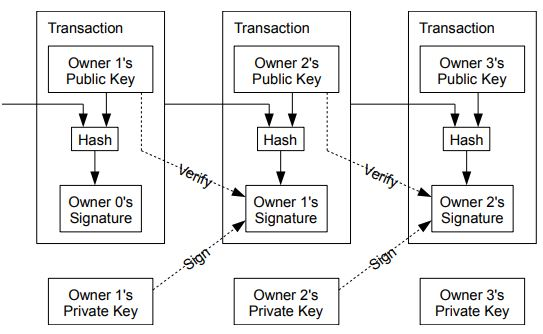
\includegraphics[scale=0.75]{immagini/cap2/1-autenticazione} 
\caption{Autenticazione della catena di transazioni}
\label{im:verifica} 
\end{figure}

%**************************************************************
\subsection{Struttura dei blocchi}
Come dice il nome, la blockchain \`e una catena di blocchi, contenenti transazioni valide. L'intera rete \`e formata da utenti chiamati \textit{nodi}, che possono essere localizzati in qualsiasi parte del pianeta. Ciascun nodo contiene il registro di tutte le transazioni effettuate nella rete fino a quel momento.
Un qualsiasi blocco contiene le seguenti informazioni~\cite{art:bc2}:
\begin{itemize} 
\item la dimensione (in byte) del blocco;
\item l'\textit{intestazione} (header) con diversi campi al suo interno, mostrati nella tab.~\ref{tab:intestazione};
\item il numero totale di transazioni. 
Ogni blocco \`e identificato in maniera univoca da un \textit{hash}, generato usando l’algoritmo crittografico di hashing sull’intestazione del blocco (per il Bitcoin, per esempio, l'algoritmo \`e SHA-256). La tab.~\ref{tab:blocco} mostra la struttura di un blocco.
\end{itemize}
\begin{table}
\centering
\begin{tabular}[t]{|c|l|}
\hline
\textbf{Campo} & \textbf{Descrizione} \\
\hline
Previous Block Hash & Hash del blocco precedente (parent block) a cui \`e collegato\\
\hline
Merkel Root & Hash della radice del merkel tree associato al blocco \\
\hline
Timestamp & Ora di creazione del blocco \\
\hline
Difficulty Target & Target usato per il PoW \\
\hline
Nonce & Numero contatore usato per il PoW \\
\hline
\end{tabular}
\caption{Struttura dell'intestazione}
\label{tab:intestazione}
\end{table}
\begin{table}
\centering
\begin{tabular}[t]{|c|l|}
\hline
\textbf{Campo} & \textbf{Descrizione} \\
\hline
Block Size & Dimensione del blocco in bytes \\
\hline
Block Header & Intestazione del blocco contenente diversi campi \\
\hline
Counter & Numero totale di transazioni registrate \\
\hline
Transactions & Transazione registrate nel blocco \\
\hline
\end{tabular}
\caption{Struttura di un blocco}
\label{tab:blocco}
\end{table}
I blocchi sono collegati ``all'indietro" (back-linked), cio\`e ognuno si riferisce al blocco precedente presente nella catena. Per questo motivo, la blockchain \`e spesso visualizzata come una pila verticale, con blocchi stratificati l’uno sopra l’altro. Questa visualizzazione, provoca l’uso di terminologie come \textit{altezza} (height) per riferirsi alla distanza dal primo blocco e \textit{top} o \textit{tip} (cima o punta) per riferirsi al blocco aggiunto più recentemente.
Ciascun blocco inoltre referenzia il blocco precedente, conosciuto anche come \textit{parent block} (blocco genitore), attraverso il campo \textit{previous block hash} dell'intestazione. La sequenza di hash che collegano ogni blocco al proprio genitore crea una catena che si collega, blocco per blocco fino al primo blocco creato, denominato \textit{genesis block}.
Una semplice rappresentazione \`e mostrata nella fig.~\ref{im:pila}.
\begin{figure}
\centering 
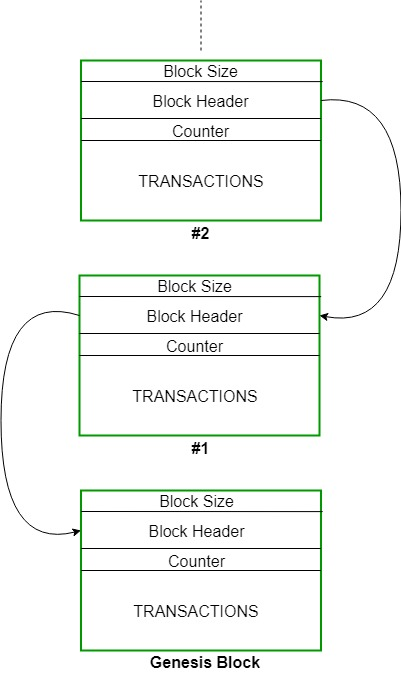
\includegraphics[scale=0.65]{immagini/cap2/2-BC-come-catena} 
\caption{Blockchain vista come una catena}
\label{im:pila} 
\end{figure}
Si supponga che un genitore venga modificato in qualsiasi modo. Allora il suo hash cambia. L’hash modificato necessita un cambio nel puntatore \textit{previous block hash} del figlio. Questo, a sua volta, causa il cambio dell’hash del figlio, che richiede il cambio nel puntatore dell’hash nipote, che a sua volta cambia il puntamento al nipote, e così via. Questo effetto a cascata assicura che, fino a quando un blocco ha tante generazioni di blocchi che lo seguono, non può essere modificato senza forzare un ricalcolo su tutti i blocchi seguenti. Visto che per questo ricalcolo servirebbe un’enorme potenza computazionale, l’esistenza di una lunga catena di blocchi fa sì che la storia più profonda della blockchain sia immutabile, che \`e una degli elementi chiave della sicurezza della blockchain~\cite{libro:bitcoin}.

%**************************************************************
\subsection{Funzionamento}
Le nuove transazioni devono per prima cose essere confermate, cio\`e bisogna verificare la loro firma digitale. Questo procedimento, lo possono fare tutti gli utenti della rete. La firma digitale, però, non offre protezione contro il \textit{double spending}, cio\`e quando un utente spende più volte delle criptovalute già spese~\cite{art:satoshi}. Per risolvere questo problema, bisogna tener conto anche dei vecchi blocchi (e quindi delle vecchie transazioni), e provare che quelli nuovi, sono legati matematicamente ai precedenti. Siccome questa verifica deve essere rigorosa e non esiste un'autorità centrale, il compito spetta ai nodi della rete (lo possono fare tutti o solo alcuni). Questi nodi specializzati, prendono il nome di \textit{minatori} (o miner) e il processo di verifica che eseguono si chiama \textit{mining}. Esso può essere diverso da criptovaluta a criptovaluta. La conferma avviene trovando il valore di hash che soddisfa una certa proprietà (procedimento chiamato \textit{proof of work}, abbreviato \textit{PoW}). Quando si trova una soluzione, il nuovo blocco \`e ritenuto valido e viene aggiunto al registro di ogni nodo. Il risultato finale \`e una catena di blocchi approvati non modificabili e in ordine cronologico.

%**************************************************************
\subsection{Mining di una criptovaluta}
Per \textit{mining} si intende quel processo svolto da un insieme di utenti della rete che, fa eseguire all'hardware di ogni utente calcoli matematici al fine di confermare il nuovo blocco ed aumentare la sicurezza della rete~\cite{sito:bitcoin}.
Questo processo ha due scopi:
\begin{itemize}
\item mantiene l’integrità e l’autenticità della blockchain, assicurando che le transazioni siano confermate solo se \`e stata usata sufficiente potenza di calcolo per il blocco che le contiene;
\item emette una quantità stabilita di nuove criptovalute (quasi come una banca centrale emette nuova moneta), che spettano al minatore che per primo le ha prodotte. A tale quantità prestabilita va a sommarsi anche il totale delle commissioni delle transazioni registrate nel blocco~\cite{art:bc2}.
\end{itemize} 
Dunque, la sicurezza della blockchain \`e resa possibile da quanti più nodi “onesti” sono presenti nella rete, in modo da rendere difficile (se non impossibile) il lavoro dei nodi “disonesti” che vogliono invece modificare il registro a loro vantaggio. 
L’onestà dei nodi \`e ``comprata” attraverso un particolare sistema di attribuzione di ricompense, che incentivano tale onestà~\cite{tesi:venezia}.
Quando arrivano delle nuove transazioni, esse vengono aggiunte a un pool temporaneo di transazioni non verificate. Questo pool, \`e memorizzato da ogni minatore. Man mano che i minatori generano un nuovo blocco, prelevano le transazioni non verificate dal pool. Esse vengono aggiunte al nuovo blocco, ordinate secondo certi criteri (ad esempio, dando priorità a quelle con commissioni maggiori). Da qui in poi, ogni minatore inizia il processo di mining di un nuovo blocco di transazioni. Nel momento in cui riceve un blocco valido da un altro minatore, capisce di aver perso la sfida. Dunque lo controlla (procedimento chiamato \textit{consenso}) e lo aggiunge alla sua blockchain. Dopodich\`e, ritenta la sfida con un nuovo blocco, creato a partire da altre transazioni e il procedimento si ripete.
Più nel dettaglio, il funzionamento del processo di mining \`e il seguente: il minatore ha come input l'intestazione del blocco nuovo e un numero, chiamato \textit{nonce} (che, tra l'altro, \`e un campo presente nell'intestazione). Il nonce \`e un numero (spesso scelto arbitrariamente) che viene utilizzato solo una volta per questo scopo e poi scartato~\cite{art:bc1}. L'input \`e rappresentato nella fig~\ref{im:input}.
\begin{figure}
\centering 
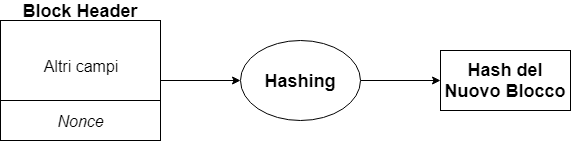
\includegraphics[scale=0.55]{immagini/cap2/3-input} 
\caption{Input utilizzato per il calcolo dell'hash del nuovo blocco}
\label{im:input} 
\end{figure}
Ora, partendo da questo input, il minatore calcola il corrispettivo hash e verifica se ha una certa proprietà/struttura definita dalla criptovaluta. Se così non fosse, cambia nonce e ritenta. Il compito del minatore, \`e dunque quello di trovare il nonce che soddisfa la proprietà. L'insieme di questi compiti matematici, prende il nome di \textit{proof of work}, abbreviato in \textit{PoW} (prova del lavoro).
La complessità del proof of work sta proprio nell'ottenere il nonce corretto, in quanto questo comporta il calcolo di un numero esponenziale di hash~\cite{art:bc2}.
Una volta che un minatore trova la soluzione per validare il blocco, manda a tutti gli altri minatori della rete:
\begin{itemize}
\item il nuovo blocco appena confermato;
\item il nonce corretto;
\item l'hash del nuovo blocco (calcolato con il nonce corretto), che \`e legato all'ultimo blocco, in quanto, per calcolarlo, \`e stato utilizzato il suo hash.
\end{itemize}
Essi, dovranno confermare che il risultato trovato \`e corretto. Se \`e così, il nuovo blocco viene aggiunto ``in cima" alla blockchain e il minatore che ha validato il blocco per primo otterrà la ricompensa. Tale verifica, chiamata anche \textit{consenso}, \`e semplice e veloce, in quanto basta calcolare un solo hash e verificare che combaci~\cite{art:bc2}.

%**************************************************************
\subsection{Numero di conferme}
Nella realtà, succede molto spesso che i minatori scelgono transazioni diverse per un blocco (scegliendo, per esempio, quelle con commissioni elevate). Quindi ognuno può lavorare su un potenziale blocco diverso che cercherà di confermare prima degli altri. Quello che succede in questo caso, \`e che si formino delle \textit{ramificazioni} nella parte finale della blockchain. Quando avvengono queste situazioni, la soluzione da adottare \`e specificata negli algoritmi delle criptovalute. Una regola molto comune, \`e quella di far continuare la blockchain sul suo ramo più lungo, mentre tutto il resto viene ignorato. Nella fig.~\ref{im:rami} \`e mostrato un esempio di blockchain ramificata, che continua sul ramo più lungo.
\begin{figure}
\centering
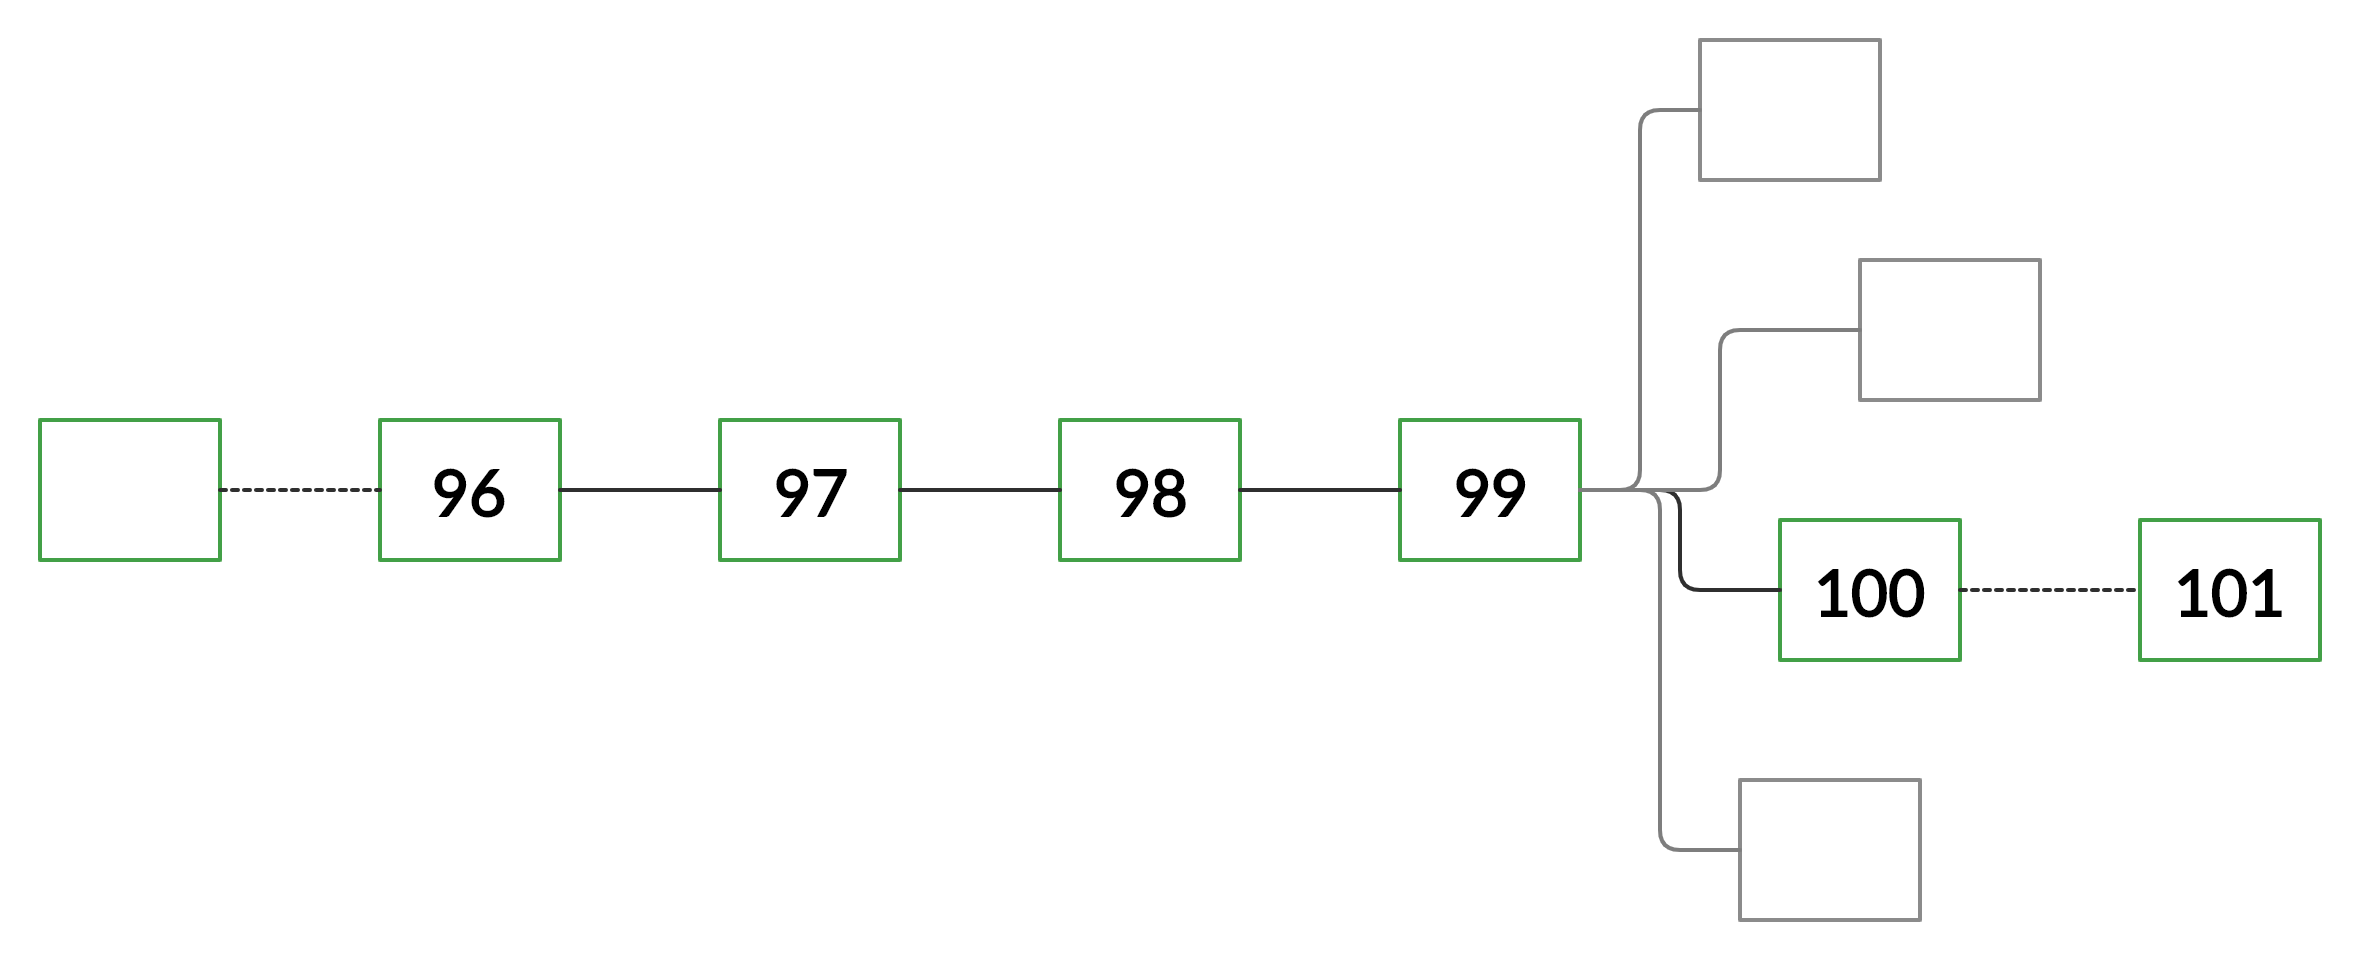
\includegraphics[scale=0.18]{immagini/cap2/3-rami} 
\caption{Esempio di blockchain ramificata}
\label{im:rami} 
\end{figure}
Basandoci sulla fig.~\ref{im:rami}, supponiamo che l’ultimo blocco confermato della blockchain sia il blocco numero 100. Ora, supponiamo che un minatore malintenzionato voglia contraffare questo blocco e quindi lo modifichi. Ovviamente, potrà apporre tale modifica solo sulla copia della blockchain che ha sul suo server. Dopodich\`e, dovrà far accettare (e quindi divulgare) la sua copia “contraffatta” al resto della rete.
Per riuscire nel suo intento, il malintenzionato dovrà:
\begin{itemize}
\item trovare un nonce per il blocco 100 che lui ha modificato, in modo che il sistema non evidenzi il suo tentativo di contraffazione;
\item aggiudicarsi la gara sul blocco 101 (perch\`e si continua sul ramo più lungo). 
\end{itemize}
In sostanza, dovrà riuscire a trovare 2 nonce (per il blocco 100 e blocco 101) prima che un qualunque altro minatore riesca a trovarne uno solo, ovvero quello per il blocco 101. 
Il tutto sarà esponenzialmente più improbabile se vorrà contraffare una transazione del blocco 99 perch\`e dovrà trovare tre nonce\dots\, e così via per i blocchi precedenti.
Per questi motivi, per misurare la sicurezza di una transazione, si indicano il numero delle conferme che ha ricevuto: ad esempio, se l’ultimo blocco confermato \`e il numero 100, allora una transazione presente nel blocco 98 si dice abbia 3 conferme, ovvero la conferma del blocco 98, quella del 99 e quella del 100.

%**************************************************************
\subsection{Esempio: Mining del Bitcoin}
Il processo di mining di un Bitcoin si basa sull'algoritmo \textit{Hashcash}~\cite{art:satoshi}. Il funzionamento \`e molto simile a quello descritto in precedenza per una criptovaluta generale. In particolare, Bitcoin utilizza \textit{SHA-256} come funzione di hash (ciò significa che l'impronta generata sarà di 256 bit). Inoltre, il minatore deve trovare quel nonce tale per cui l'hash di output inizi con $n_z$ zeri, dove $n_z$ sono i bit più significativi~\cite{art:bc2}.
Per vedere se il nonce utilizzato \`e quello corretto, il minatore controlla se l'hash risultante \`e minore o uguale di un certo valore di 256 bit, chiamato \textit{target} (che tutti i minatori conoscono). Se \`e più piccolo, significa che l'output aveva almeno uno zero inziale in più rispetto al target e dunque il minatore ha trovato la soluzione; altrimenti, il nonce viene incrementato di uno e si riprova (il nonce parte da zero). Il valore target viene ricalcolato ogni 2016 blocchi (circa due settimane). Ad esempio, se il target corrente fosse di $00000111$ e l'hash di output $001110010$, il minatore non avrebbe trovato una soluzione valida, perch\`e il target ha 5 zeri iniziali e il risultato solo 2; il minatore deve aumentare progressivamente il nonce ad ogni nuovo tentativo, finch\`e il risultato non inizia con almeno 6 zeri~\cite{tesi:venezia}. La fig~\ref{im:flow} mostra il diagramma a blocchi del processo di mining del Bitcoin.
\begin{figure}
\centering
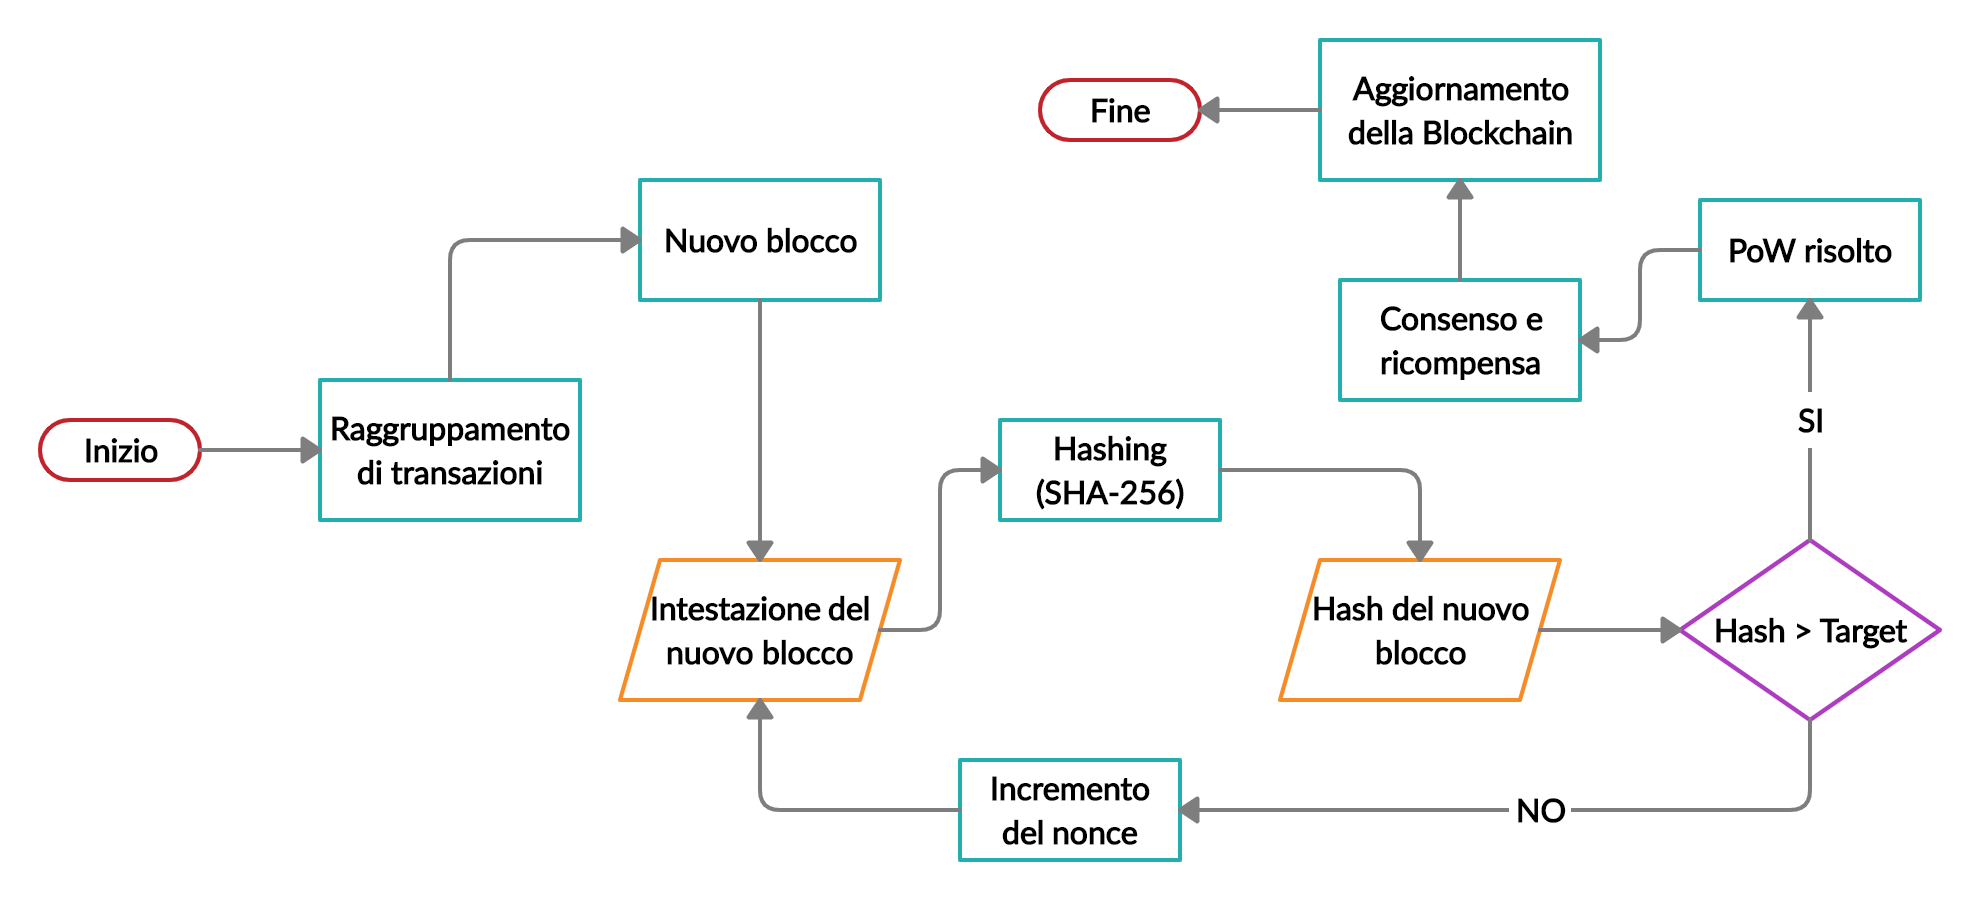
\includegraphics[scale=0.23]{immagini/cap2/4-flow} 
\caption{Diagramma a blocchi del processo di mining del Bitcoin}
\label{im:flow} 
\end{figure}
Il lavoro medio richiesto \`e esponenziale rispetto al numero di zeri. In più, SHA-256 richiede un \textit{hash rate}% 
\footnote{Per \textit{hash rate} si intende l'unità di misura della potenza di elaborazione della rete di una criptovaluta, cio\`e quanti calcoli matematici riesce ad eseguire in un certo tempo. Ad esempio, quando la rete raggiunge un hash rate di 10 TH/s, significa che può realizzare un trilione di calcoli al secondo.~\cite{sito:bitcoin}} elevato, di giga hashes al secondo (GH/s) o superiore~\cite{art:bc1}. 
Il tempo medio necessario per estrarre un blocco Bitcoin con SHA-256 \`e circa di 10 minuti~\cite{sito:bitcoin}.
Il procedimento di proof of work del Bitcoin \`e identico a quello descritto precedentemente per una criptovaluta generale.
Il minatore che ha risolto per primo il blocco, verrà premiato con dei Bitcoin. Il premio varia in base al numero di Bitcoin estratti. Poich\`e c'\`e n\`e un numero limitato, i premi diminuiscono della metà dopo ogni 210.000 blocchi estratti (circa ogni 4 anni). A partire da agosto 2018, i minatori vengono premiati con 12,5 Bitcoin. Nei primi anni, cio\`e nel 2009, i minatori guadagnavano 50 Bitcoin~\cite{art:bc2}.
Oltre alla ricompensa ottenuta dal mining, i minatori ricevono anche un importo chiamato \textit{commissione di transazione} per ogni transazione confermata che aggiungono alla blockchain~\cite{art:bc1}.
Per convenzione, una transazione che riceve 6 conferme (cio\`e sopra il suo blocco ne vengono aggiunti altri 5) viene considerata sicura al 100\%.



\section{Catena di Markov}
\label{sottocap:teo-code}
Una \textit{\textbf{catena di Markov}} \`e un processo stocastico avente una proprietà caratterizzante, chiamata \textit{proprietà di Markov}~\cite{libro:tele}.  Il processo, che può essere a tempo continuo o a tempo discreto, \`e determinato da una successione di variabili aleatorie $\{X_w\}$, che prendono valori in un insieme $S$, detto \textit{spazio degli stati}. Esso può essere finito o al più infinito numerabile. 
L’indice $w$ di $\{X_w\}$ indica il \textit{tempo}, mentre i possibili valori della successione prendono il nome di \textit{stati} del processo.
Al trascorrere del tempo, il processo può “saltare“ da uno stato all’altro. Se ad un certo istante $w$ si trova in uno stato $i$ ed all’istante successivo ($w+1$ se \`e discreto oppure $w+u$ se \`e continuo) si trova in uno stato $j \neq i$, si dirà che c’\`e stata una \textit{transizione}.
Siccome i processi coinvolti sono stocastici, i calcoli coinvolgeranno le probabilità. Le più importanti sono le cosiddette \textit{probabilità di transizione}. Per il \textit{tempo discreto} valgono:
\begin{equation}P_{i,j}(k)=P[X_{n+k}=j | X_n=i]\end{equation} 
che indica la probabilità di trovarsi nello stato $j$ al tempo $n+k$ sapendo di essere nello stato $i$ al tempo $n$. In questo caso, $k$ indica il \textit{numero di step} per andare dallo stato $i$ allo stato $j$.\\
Per il \textit{tempo continuo} invece, valgono:
\begin{equation}P_{i,j}(u)=P[X(t_0+u)=j | X(t_0)=i]\end{equation} 
che indica la probabilità di trovarsi nello stato $j$ al tempo $t_0+u$ sapendo di essere nello stato $i$ al tempo $t_0$. In questo caso, $u$ indica l'\textit{intervallo temporale} per andare dallo stato $i$ allo stato $j$.\\
Si dirà che queste probabilità sono $stazionarie$ se dipendono solo dalla lunghezza temporale $k$ o $h$ (a seconda che il tempo sia discreto o continuo) e non dai singoli istanti $n$ o $t_0$. Le relative catene di Markov, invece, si diranno \textit{omogenee}. I processi che si andranno a sviluppare nei capitoli successivi, sono tutti di questo tipo.

%**************************************************************
\subsection{Proprietà di Markov}
La proprietà di Markov per un processo a tempo discreto \`e sintetizzata nella seguente formula:
\begin{equation}\label{eq:pr1}P[X_{n_k}=\sigma_k | X_{n_{k-1}}=\sigma_{k-1},\dots,X_{n_0}=\sigma_0]=P[X_{n_k}=\sigma_k | X_{n_{k-1}}=\sigma_{k-1}].\end{equation}
Mentre, per un processo a tempo continuo, vale:
\begin{equation}\label{eq:pr2}P[X_{t_n}=\sigma_n | X_{t_{n-1}}=\sigma_{n-1},\dots,X_{t_0}=\sigma_0]=P[X_{t_n}=\sigma_n | X_{t_{n-1}}=\sigma_{n-1}],\end{equation}
dove i $\sigma_i$ sono elementi appartenenti allo spazio di stato $S=\{0,1,2,\dots\}$.\\
L’interpretazione della proprietà di Markov \`e la seguente. Consideriamo:
\begin{itemize}
\item l'istante $n_{k-1}$ (o nel continuo $t_{n-1}$) come il ``presente" del processo;
\item gli istanti $n_0, n_1, \dots, n_{k-2}$ (o nel continuo $t_0, t_1, \dots, t_{n-2}$) come il ``passato" del processo;
\item l'istante $n_k$ (o nel continuo $t_n$) come il ``futuro" del processo.
\end{itemize}
Dunque, le equazioni~\eqref{eq:pr1} e~\eqref{eq:pr2} ci dicono dice che la conoscenza del ``passato" del processo non predice la sua evoluzione futura dallo stato $\sigma_{k-1}$ in cui si trova al momento. Perciò, \`e possibile ``dimenticarsi" della storia passata, conoscendo esclusivamente lo stato presente.

 %File in cui verrà scritto il capitolo

\clearpage{\pagestyle{plain}\cleardoublepage} %Comando per iniziare il capitolo su pagina dispari
\chapter{Analisi del modello M/G/1} %Nome capitolo
\label{cap:MG1} %Label per creare riferimenti al capitolo
Il modello M/G/1 simboleggia un sistema che ha un solo servitore, in cui gli arrivi sono markoviani (o senza memoria), mentre il servizio segue una distribuzione generica $F_y(a)$. Per fissare le idee, diciamo che il tasso degli arrivi \`e pari a $\lambda$, mentre il tasso di servizio \`e pari a $\mu$.
La markovianità degli arrivi \`e giustificata dal fatto che in una rete grande, le possibili sorgenti di transazione sono molte e indipendenti; mentre la stazionarietà/omogeneità \`e giustificata dal fatto che il comportamento della rete \`e tempo invariante. La statistica dei tempi di inter-arrivo \`e esponenziale perch\`e \`e conseguenza della poissonianità e omogeneità.
Il fatto che il sistema abbia un solo servitore, non significa che anche il numero di minatori dell'intera rete sia uno, ma significa che la stessa transazione (che \`e il cliente del sistema) viene servita da tutti gli $m$ minatori. Dunque, in termini di teoria delle code, \`e come avere un sistema formato da una sola coda in cui il cliente viene servito da un'unica entità composta da $m$ minatori che la servono contemporaneamente.
Il modello M/G/1 \`e utilizzato in letteratura per il calcolo dei tempi di conferma delle transazioni e dei ritardi e dello studio dei fattori che li influenzano, come ad esempio la dimensione del blocco o il numero di transazioni.

%*****************************************************************
\section{Rappresentazione come catena di Markov}
Il modello M/G/1 si può analizzare facilmente se lo si rappresenta come una catena di Markov. Per farlo, però, bisogna dimostrare la prorpietà di Markov e trovare lo stato e la sua statistica. Fatto questo, poi, si possono ricavare le statistiche e i momenti di tutte le metriche. Si inizia considerando il numero totale di clienti $x(t)$ nel sistema negli istanti immediatamente successivi alla $n$-esima partenza dal sistema, denominati $t_n^+$%
.\footnote{Il termine \textit{clienti} \`e usato per questo modello in maniera generale. Infatti, ci si può riferire ai clienti sia come transazioni sia come blocchi.} Indicando con $x_n:= x(t_n^+)$ il numero di clienti nel sistema immediatamente dopo il verificarsi della $n$-esima partenza, possiamo scrivere le seguenti relazioni che ne specificano la dinamica~\cite{libro:tele}:
\begin{itemize}
\item se la partenza $n$-esima lascia il sistema vuoto, prima che si verifichi una nuova partenza, \`e necessario attendere l’arrivo di un cliente e la fine del suo tempo di servizio. Supponiamo che in questo lasso di tempo, arrivi un numero di clienti pari alla variabile aleatoria $v_n$. Dunque, un instante dopo la partenza $n$-esima, il numero totale di clienti diventa pari a $v_n$. In formula: \begin{equation} x_{n+1}=v_n \end{equation}
\item se dopo la partenza $n$-esima il sistema non \`e vuoto, il prossimo cliente in coda accede al servizio e si aggiungono poi $v_n$ clienti al sistema. Dunque, dopo la partenza, avremo $x_n-1$ clienti rimanenti e in più i $v_n$ appena arrivati. In formula: \begin{equation} x_{n+1}=x_n-1+v_n \end{equation}
Possiamo unificare le due equazioni precedenti utilizzando la funzione indicatrice:
\begin{equation}\label{eq:chi}\chi \{x_n>0\}=\begin{cases} 1 & \text{se}\quad x_n>0\\ 0 & \text{se}\quad x_n=0 \end{cases}\end{equation}
ottenendo dunque:
\begin{equation}\label{eq:stato} x_{n+1}=x_n+v_n-\chi \{x_n>0\}. \end{equation}
\end{itemize}
Ora, per poter dire che il sistema M/G/1 evolve secondo una catena di Markov, bisogna dimostrare che la descrizione statistica fatta per gli istanti $t_n^+$, valga \textit{per ogni} istante di osservazione. 
Un modo per dimostrarlo \`e il seguente. Si può notare che, asintoticamente, il numero $x_n$ di clienti nel sistema subito dopo una partenza, \`e distribuito come $x(\tau_m^-)$, che \`e il numero di clienti nel sistema appena prima l'arrivo di un nuovo cliente. Dopodich\`e, si può sfruttare la proprietà PASTA, che dice che gli arrivi poissoniani ``vedono" davanti a loro, la distribuzione asintotica dello stato $x(t)$. Dunque, $x(\tau_m^-)$ \`e distribuita come $x(t)$ per $t \to \infty$. Ma allora, se asintoticamente $x_n$ \`e distribuita come $x(\tau_m^-)$ che, a sua volta, \`e distribuita come $x(t)$, vale che per $n \to \infty$, $x_n$ converge alla distribuzione di $x(t)$. In conclusione, in regime stazionario e in qualsiasi istante di osservazione, si ha un'unica descrizione statistica dello stato~\cite{libro:tele}.

%*****************************************************************
\section{Calcolo del tempo medio di attesa in coda}
Ora, si vuole riportare il calcolo del tempo medio di attesa in coda $E[T_Q]$, che in ambito criptovalute, viene visto come il \textit{ritardo} del tempo di conferma di una transazione. Per tutti gli altri momenti delle metriche, si consiglia di vedere~\cite[586-587]{libro:tele}.
Viene sfruttata la tecnica \textit{tagged-job}, nella quale si ``tagga" un arrivo arbitrario e si ragiona sul tempo speso in coda proprio da questo arrivo selezionato~\cite{libro:tempo-MG1}. Si ipotizza che tutte le variabili in gioco siano i.i.d.
Verrà utilizzata la seguente notazione:
\begin{itemize}
\item $\rho=\frac{\lambda}{\mu}=$ fattore di carico;
\item $T_Q=$ tempo in coda;
\item $N_Q=$ numero clienti in coda;
\item $N_Q^A=$ numero clienti in coda visti dal cliente ``taggato";
\item $S=$ tempo di servizio $\implies$ $E[S]=\frac{1}{\mu}$;
\item $S_i=$ tempo di servizio $i$-esimo cliente;
\item $S_e=$ tempo di servizio visto dal cliente ``taggato".
\end{itemize}
Allora:
\begin{subequations}\begin{align}E[T_Q] & \notag =E[\text{tempo di servizio dei clienti in coda prima del ``tag"}]\\ \notag & +E[\text{tempo di servizio residuo del cliente in servizio}]= \\ \notag
&=E[\sum_{i=1}^{N_Q^A} S_i]+E[\text{tempo di servizio residuo del cliente in servizio}]=\\ \notag
&\underset{\text{indip.}}{=} E[N_Q^A] E[S] + P[\text{unico servitore \`e impegnato}] E[S_e]=\\ 
&\label{eq:tempo-coda} \underset{\text{PASTA}}{=} E[N_Q] E[S] + \rho E[S_e]=\\ \notag
&\underset{\text{Little}}{=} E[T_Q] \lambda E[S] + \rho E[S_e]=\\ \notag
&=\rho E[T_Q] + \rho E[S_e]=\\ 
&= \frac{\rho}{1-\rho} E[S_e]. \end{align}\end{subequations}

%*****************************************************************
\section{Analisi della statistica del ritardo}
Nell'articolo~\cite{art2:MG1}, si parla dei fattori che impattano i ritardi delle transazioni Bitcoin sfruttando la teoria delle code. Per \textit{ritardo} si intende quell'intervallo temporale che la transazione deve attendere prima di essere scelta per far parte di un blocco. Utilizzando la nomenclatura della teoria delle code e considerando le transazioni come clienti, il ritardo equivale al tempo medio di attesa in coda, che in questo caso viene chiamata in gergo \textit{mining pool}. In~\cite[sez. 4]{art2:MG1} sono scritti i parametri considerati. Vengono riportati quelli più rilevanti:
\begin{itemize}
\item $\lambda$ \`e il tasso di arrivo di un gruppo di transazioni;
\item $\lambda_B$ \`e il tasso con cui vengono minati i blocchi (misurato in $blocchi/s$);
\item ogni blocco contiene in media $\tau$ transazioni;
\item $\lambda=\lambda_B \tau$ \`e il tasso di servizio delle transazioni;
\item $B$ \`e il tempo che intercorre tra la conferma di due blocchi (tempo inter-blocco). Inoltre vale che $E[B]=\frac{1}{\lambda_B}$;
\item $D$ \`e il ritardo di una transazione. In particolare, $D_{i,j}$ indica il tempo dall’ istante della conferma della $j$-esima transazione nel blocco $i$ fino all’istante di conferma dell'intero blocco.
\end{itemize}
Dopodich\`e, sfruttando la tecnica \textit{tagged-job}, gli autori hanno affermato che:
\begin{equation}\label{eq:ritardo} E[D]=\alpha E[B] + E[B_r], \end{equation} 
dove:
\begin{itemize}
\item $E[B_r]$ \`e il tempo medio residuo del blocco in servizio;
\item $\alpha$ denota il numero medio di blocchi che un utente deve attendere prima che la sua transazione sia confermata. Una transazione \`e confermata quando il suo blocco \`e aggiunto alla blockchain e poi vengono aggiunti altri blocchi sopra di esso (blockchain come pila, fig.~\ref{im:pila} della sottosez.~\ref{sottocap:bc-cripto}). Questo parametro, viene poi calcolato tramite simulazioni.
\end{itemize}
Infatti, la formula~\eqref{eq:ritardo} dice che il ``tag", deve tener conto del tempo medio residuo del blocco davanti a lui, ma anche del tempo medio che un altro blocco si aggiunga sopra al suo nella blockchain, perch\`e così conferma il suo blocco.
Si può notare che la formula~\eqref{eq:ritardo} \`e molto simile alla formula~\eqref{eq:tempo-coda} ricavata sopra per un sistema M/G/1.
Dopodich\`e, in~\cite[sez. 5]{art2:MG1}, gli autori hanno condotto tre simulazioni, scegliendo altrettanti intervalli temporali e usando le statistiche del sito Bitcoin. In tutte e tre le prove, si può notare che il numero delle transazioni con commissioni medie elevate, \`e maggiore rispetto al numero di quelle con commissioni basse e dunque, le prime vengono confermate in un tempo più corto (in media 30 minuti). Questo risultato \`e scontato, perch\`e i minatori cercano sempre il maggior profitto (il tutto \`e riportato nella tab. 3~\cite[sottosez. 5.1]{art2:MG1}). Inoltre, gli autori hanno trovato tre valori del parametro $\alpha$, il cui risultato \`e $\alpha<1$. La conclusione di ciò, \`e che per avere una conferma attendibile della transizione, basta che il blocco che la contiene, venga inserito nella blockchain (non serve aspettare l'aggiunta di altri blocchi).

%*****************************************************************
\section{Analisi della statistica dei tempi di conferma}
Nell'articolo~\cite{art3:MG^B1}, invece, viene sviluppato un modello per il Bitcoin, nominato M$/G^B$/1, la cui particolarità \`e il \textit{batch service}. Un sistema di questo tipo, funziona esattamente come il tradizionale M/G/1 in cui però, se al termine di un servizio sono presenti clienti in coda, essi vengono serviti in gruppo (batch). La dimensione del batch \`e limitata e costante. In questo caso specifico, i clienti sono le transazioni, che vengono processate in blocco quando il minatore \`e libero. Gli autori di~\cite{art3:MG^B1}, inoltre, assumono che se le transazioni arrivano nel sistema quando \`e già in atto un processo di mining, esse vengono aggiunte al blocco in servizio solo se la sua dimensione \`e più piccola della massima dimensione possibile. Viene indicato con $b$ il numero massimo di transazioni che può contenere un blocco. Il calcolo di $b$ \`e stato fatto studiando le statistiche su vari intervalli temporali. Bitcoin usa come dimensione di blocco circa 1 MByte e all’interno si trovano in media 1750,27 transazioni (per maggiori dettagli si veda~\cite[sottosez. 3.2]{art3:MG^B1}). Nel modello di~\cite{art3:MG^B1}, \`e usato $b=2000$ per riferisi ad un blocco di 1 MByte.
In~\cite{art3:MG^B1}, gli autori studiano il tempo medio di conferma delle transazioni (indicato con $E[T]$ o TCT) considerando anche le priorità che esse hanno, a differenza di~\cite{art2:MG1}, dove quest'ultima non veniva presa in considerazione. La priorità può essere di qualsiasi tipo. Spesso, si dice che una transazione ha un'alta priorità se ha una commissione elevata. Nell'articolo, invece, viene data alta priorità se la transazione ha un alto importo. 
Inoltre, \`e riportato che le transazioni che hanno un maggiore pagamento sono quelle che vengono scelte per prime dai minatori e quindi, il loro tempo di conferma sarà più piccolo. Lo studio \`e stato condotto tramite simulazioni, dividendo le transazioni in due classi: la \textit{classe H} per quelle che hanno un valore maggiore di 1 BTC e la \textit{classe L} per quelle il cui valore \`e minore. 
Il motivo della scelta di questo valore per la divisione in classi non \`e illustrata nell'articolo. Inoltre, in~\cite[sottosez. 4.2]{art3:MG^B1}, la \textit{classe L} viene divisa ancora in altre due classi, \textit{L1} ($importo<0.01~BTC$) e \textit{L2} ($importo \ge 0.01~BTC$). In~\cite[fig. 1]{art3:MG^B1} \`e mostrata la percentuale di transazioni (con relativa classe) presente nel blocco in un arco temporale di due anni. La figura \`e poco chiara, perch\`e non si vede il contributo della \textit{classe L1}. Nemmeno in questa sottosezione vengono spiegati i motivi delle scelte dei valori BTC per la divisione in classi. Ritengo che la divisione in \textit{L1} e \textit{L2} serva per far vedere (tramite la fig.1) che negli ultimi anni, ci sono state più transazioni di \textit{L2} che di \textit{L1} (oltre a quelle di \textit{H}). Però, proprio perch\`e si vogliono analizzare le statistiche dei tempi dei micro-pagamenti, gli autori avrebbero potuto studiare anche \textit{L1} e \textit{L2} oltre che \textit{H} e \textit{L}.
Questo articolo, quindi, ci dice che, oltre alle commissioni elevate (studio condotto da~\cite{art2:MG1}), un altro parametro da tener in considerazione per velocizzare i tempi di conferma, \`e il valore del pagamento che riporta la transazione. In realtà, questi due parametri sono collegati tra loro, perch\`e si suppone che chi trasferisce grandi quantità di criptomoneta, possa pagare anche delle maggiori commissioni. \\
In conclusione,~\cite{art3:MG^B1} mostra i seguenti casi:
\begin{itemize}
\item \textit{senza classe}: mostrato in fig.~\ref{im:confronto-classless}; il caso più comune \`e quello di $b=2000$, in cui il tempo di conferma cresce rapidamente se $\lambda >3$. Raddoppiando $b$, il tempo effettivamente diminuisce, ma con $b=8000$, abbiamo che il sistema diventa instabile se $\lambda>12$. Ora, in termini di $\lambda$ non c’\`e una grande variazione (si passa da 3 a 12), cio\`e si rimane sullo stesso ordine di grandezza. Questo fa capire che aumentare la dimensione massima del blocco non \`e un metodo efficace per mitigare considerevolmente il tempo di conferma;
\begin{figure}[!ht]
\centering 
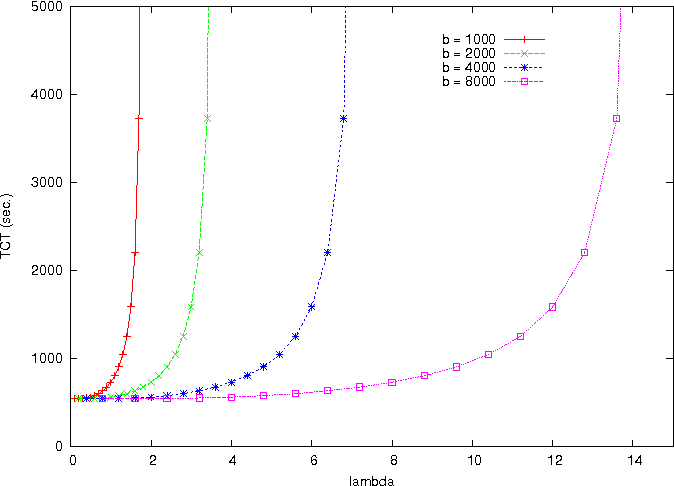
\includegraphics[scale=0.55]{immagini/Fig5-M-GB-1} 
\caption{Tempo medio di conferma delle transazioni (TCT): caso \textit{senza classe}~\cite[fig. 5]{art3:MG^B1}}
\label{im:confronto-classless} 
\end{figure}
\item \textit{classe L e H}: mostrato in fig.~\ref{im:confronto-classLH}; ciascuna classe ha un tasso degli arrivi diverso, rispettivamente $\lambda_L$ e $\lambda_H$. Il grafico mostra il tempo medio in funzione di $\lambda_L$ tenendo costante $\lambda_H$ al valore $\lambda_H=0.2535592656$ (valore calcolato a partire dalle statistiche fornite nel sito Bitcoin). I risultati mostrano quello che ci si aspettava, ovvero il tempo di conferma \`e minore per le transazioni di classe H. Anche in questo caso, aumentare la dimensione dei blocchi non riduce considerevolmente il problema (fig.~\ref{im:confronto-classLH}).
\begin{figure}[!ht]
\centering 
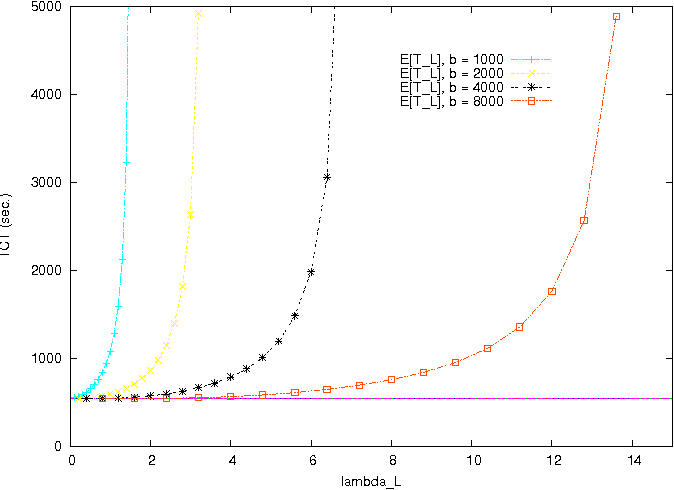
\includegraphics[scale=0.70]{immagini/Fig6-M-GB-1} 
\caption{Tempo medio di conferma delle transazioni (TCT): caso \textit{classe L e H}~\cite[fig. 6]{art3:MG^B1}}
\label{im:confronto-classLH} 
\end{figure}
\end{itemize}

%*****************************************************************
\section{Analisi del modello M/D/1}
Il modello M/D/1 \`e un caso particolare di M/G/1, dove il tempo di servizio \`e costante: $y=T$~\cite{libro:tele}.
La statistica del tempo di servizio $y$ \`e la seguente:
\begin{equation}p_y(a)=\delta(a-T), \quad m_y=T, \quad \sigma_y^2=0. \end{equation}
Gli arrivi rimangono un processo poissoniano con tasso $\lambda$.
Per i calcoli dei momenti delle metriche, si consiglia di vedere~\cite[590]{libro:tele}.\\
La scelta del tempo di servizio \`e un compromesso tra i seguenti criteri:
\begin{itemize}
\item non deve essere troppo grande, perch\`e in tal caso, un utente malintenzionato che ha appena speso le sue criptovalute, potrebbe in quel tempo sfruttarne la vulnerabilità e fare un double-spending; 
\item non essere troppo corto, perch\`e la soluzione del PoW deve essere tale da non poter essere truccata e, se si avesse a disposizione poco tempo, questo rischio potrebbe verificarsi perch\`e verrebbe scelta una soluzione ``banale".
\end{itemize}
 %File in cui verrà scritto il capitolo

\clearpage{\pagestyle{plain}\cleardoublepage} %Comando per iniziare il capitolo su pagina dispari
\chapter{Analisi del modello M/M/1} %Nome capitolo
\label{cap:MM1} %Label per creare riferimenti al capitolo
Il modello M/M/1 \`e un caso particolare di M/G/1, in cui gli arrivi e il servizio sono markoviani (o senza memoria). I tempi inter-arrivo sono variabili aleatorie esponenziali con tasso $\lambda$. Stessa cosa dicasi per il servizio, con la differenza che i tempi hanno tasso $\mu$.
Per i calcoli dei momenti delle metriche, si consiglia di vedere~\cite[546-552]{libro:tele}.\\
Nell'articolo~\cite{art:MM1}, si utilizza un sistema M/M/1 per calcolare il tempo totale di conferma di un blocco, che \`e pari alla somma del tempo di generazione (tempo impiegato dal processo di mining) e il tempo dovuto al consenso e all'aggiunta nel registro. 
Questo articolo, però, \`e poco rigoroso nel presentare le ipotesi e i procedimenti matematici che portano ai risultati finali. Infatti, le ipotesi si basano su quelle dell'articolo~\cite{art4:GM1}, in cui si fa riferimento al modello G/$M^B$/1, che ha la particolarità di avere un \textit{batch service}. Questa ipotesi, non viene specificato in~\cite{art:MM1}. Mentre, per quanto riguarda i procedimenti matematici, dall'eq. 6 in~\cite[sez. 3]{art:MM1}, viene utilizzato il parametro $m$, che viene definito come il \textit{numero di servitori nel sistema}. Inoltre, dopo l'eq. 7 in~\cite[sez. 3]{art:MM1}, viene posto $m=2$ senza specificare il motivo di tale scelta.

%**************************************************************
\section{M/M/1 vs m$\times$M/M/1}
Il modello che più si addice alla descrizione del processo di mining \`e m$\times$M/M/1, ovvero un modello in cui ci sono $m$ minatori, i quali hanno ciascuno una coda M/M/1. Se supponiamo che ogni coda abbia un tasso degli arrivi pari a $\lambda$ e un tasso di servizio pari a $\mu$, allora il modello complessivo \`e ancora markoviano e ha tassi rispettivamente pari a $\frac{\lambda}{m}$ e $\frac{\mu}{m}$.
Per osservare le prestazioni dei due modelli, \`e utile confrontare i loro tempi medi totali $m_s$, che sono pari a~\cite[564]{libro:tele}:
\begin{itemize}
\item per M/M/1
\begin{equation}m_{s_1}=\frac{1}{\mu - \lambda}\end{equation}
\item per m$\times$M/M/1
\begin{equation}m_{s_2}=\frac{m}{\mu - \lambda}\end{equation}
\end{itemize}
Nella fig.~\ref{im:confronto} \`e mostrato il grafico che confronta le prestazioni dei due modelli, assumendo $m=20$ e $\mu=1$.
\begin{figure}
\centering 
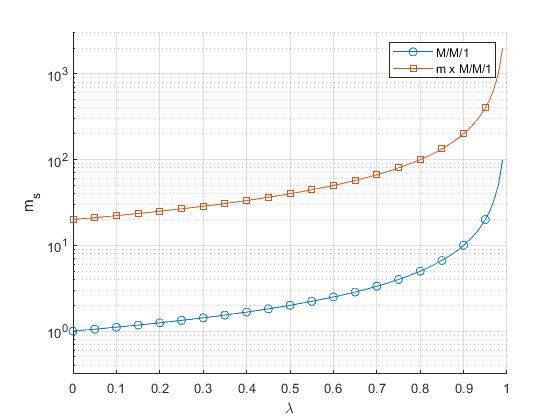
\includegraphics[scale=0.76]{immagini/confronto} 
\caption{Tempo medio di sistema $m_s$ in funzione del tasso degli arrivi $\lambda$ dei due modelli, assumendo $m=20$ e $\mu=1$}
\label{im:confronto} 
\end{figure}
Il grafico mostra l'andamento del tempo medio totale $m_s$ in funzione del tasso degli arrivi $\lambda$. Si può notare che m$\times$M/M/1 \`e la soluzione peggiore in quanto, avendo $m$ minatori che lavorano in parallelo, \`e altamente probabile che qualcuno di loro sia impegnato e qualcun altro non lo sia. Nel caso M/M/1, invece, la coda \`e unica e quindi l'unico minatore che c'\`e, rimane sempre impegnato finch\`e \`e presente qualcuno in coda. Dunque, una transazione (o un blocco) richiede un tempo complessivo maggiore con il modello m$\times$M/M/1 perch\`e, oltre ad aspettare in coda, deve attendere un tempo medio più lungo in servizio perch\`e, per ipotesi, il minatore \`e lento (ha un tasso di servizio pari a $\frac{\mu}{m}$ anzich\`e $\mu$).

%**************************************************************
\section{Analisi del processo delle partenze}
Un altro vantaggio dell'utilizzo del modello M/M/1, risiede in un teorema che si riferisce al processo delle partenze da un sistema M/M/1 stabile. Questo teorema \`e il seguente.
\begin{teorema}[di Burke] 
Il processo delle partenze da un sistema M/M/1 stabile \`e poissoniano di parametro $\lambda$.
\end{teorema}
Il fatto che il tasso di uscita sia $\lambda$ \`e dovuto alla stabilità del sistema. Il teorema di Burke dice una cosa più forte, ovvero che il processo delle uscite \`e poissoniano, quindi senza memoria. Questa proprietà può essere utilizzata per descrivere, sempre con un modello M/M/1, il \textit{consenso}, ovvero quel processo che avviene dopo il mining. Quindi, possiamo rappresentare i due processi di mining e consenso come una \textit{cascata di due code M/M/1 stabili e indipendenti}, in cui valgono tutte le proprietà già note sui singoli sistemi. Questo, \`e sicuramente un beneficio rispetto all'utilizzo di altri modelli, nel caso in cui si voglia analizzare (indipendentemente dal mining) anche il consenso.
 %File in cui verrà scritto il capitolo

\clearpage{\pagestyle{plain}\cleardoublepage} %Comando per iniziare il capitolo su pagina dispari
\chapter{Conclusioni} %Nome capitolo
\label{cap:conclusioni} %Label per creare riferimenti al capitolo
In questa tesi, si sono volute analizzare le statistiche dei tempi di conferma delle transazioni e gli aspetti che le influenzano. Inoltre, si sono confrontati i risultati degli articoli presenti in letteratura per avere delle soluzioni più ampie. In particolare, si \`e visto che:
\begin{itemize}
\item per M/G/1, l'analisi risulta più completa considerando un \textit{batch service} anziche un servizio normale. Per questo modello, si sono studiati i fattori che impattano nei tempi di conferma e nei ritardi delle transazioni, concludendo che transazioni con alte commissioni o elevati importi, hanno dei tempi minori. Nel caso particolare di M/D/1, la durata del tempo di servizio \`e un compromesso dovuto alle possibili vulnerabilità che scaturiscono nel caso di tempi troppo lunghi o troppo corti;
\item per M/M/1, c'\`e il vantaggio di poter studiare con lo stesso modello anche il processo del consenso; inoltre, in termini di prestazioni temporali, \`e preferibile un'unica coda M/M/1 con tasso di servizio $\mu$ anzich\`e $m$ code con tasso $\frac{\mu}{m}$ ciascuna.
\end{itemize}
Lo studio delle criptovalute \`e tutt'ora un tema aperto, che può portare molti spunti interessanti per il futuro, soprattutto se un giorno, si decidesse di passare dai contanti alle criptomonete. La quasi totalità degli articoli presenti in letteratura, approfondisce soprattutto il processo di mining, che indubbiamente \`e il processo alla base delle monete digitali. Per studi futuri, si può pensare di ragionare anche sul processo del consenso, integrando lo studio con altri modelli di code.
 %File in cui verrà scritto il capitolo

\clearpage{\pagestyle{plain}\cleardoublepage}
\nocite{*}
\printbibliography[heading=bibintoc]


\end{document}
